\section{Embedded Systems -- Allgemein}
\subsection{Definition}

Ein Embedded System...

\begin{itemize}
    \item ist ein System, das einen Computer beinhaltet, selbst aber kein Computer ist
    \item besteht üblicherweise aus Hardware (Mechanik, Elektronik) und Software
    \item ist sehr häufig ein Control System (Steuerung, Regelung)
\end{itemize}

\vspace{0.2cm}

Ein Embedded System beinhaltet typischerweise folgende Komponenten:

\begin{minipage}[t]{0.15\columnwidth}
    \begin{itemize}
        \item Sensoren
        \item Aktoren
    \end{itemize}
\end{minipage}
\hfill
\begin{minipage}[t]{0.3\columnwidth}
    \begin{itemize}
        \item Mikrocomputer
        \item Software (Firmware)
    \end{itemize}
\end{minipage}
\hfill
\begin{minipage}[t]{0.45\columnwidth}
    \begin{itemize}
        \item Hardware (Mechanik, Elektronik)
    \end{itemize}
\end{minipage}


\subsubsection{Charakterisierung von Embedded Systems}

Embedded Systems können \textbf{(müssen aber nicht)} folgende Eigenschaften haben:

\begin{outline}
    \1 \textbf{reactive systems:}  Reaktive Systeme interagieren mit ihrer Umgebung
    \1 \textbf{real-time systems:} Echtzeitsysteme haben nebst funktionale Anforderungen auch definierbaren zeilichen Anforderungen zu genügen
    \1 \textbf{dependable systems:} Verlässliche Systeme sind Systeme, welche (sehr) hohe Zuverlässigkeitsanderungen erfüllen müssen
    \1 \textbf{Weitere (häufige) Anforderungen:} 
        \2 kleiner Energieverbrauch
        \2 kleine physikalische Abmessungen
        \2 Lärm, Vibration, etc.
\end{outline}


\subsubsection{Typischer Aufbau}

\textbf{Ein gutes Design beinhaltet unterschiedliche Abstraktionsschichten \textrightarrow\ Layer} \\
\textrightarrow\ Siehe Abschnitt \ref{Hardware Abstraction Layer (HAL)}

\begin{center}
    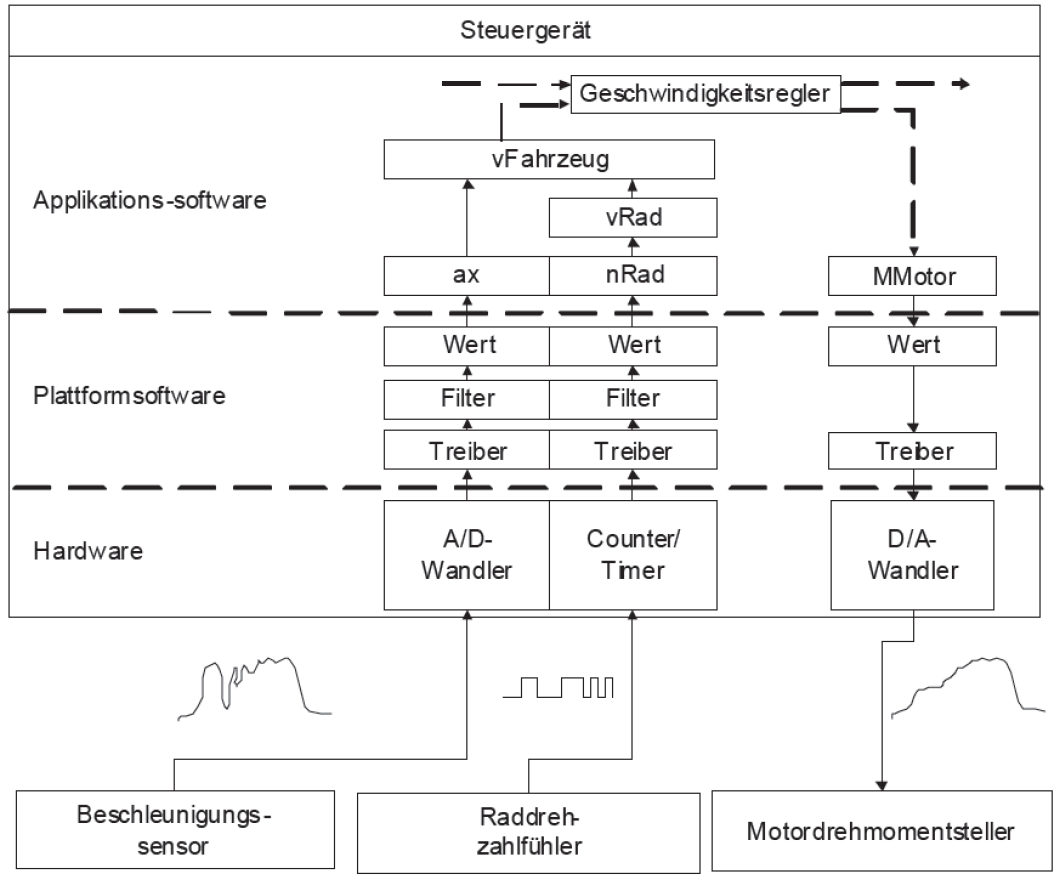
\includegraphics[width=0.8\columnwidth]{images/embedded_system_aufbau_schichten.png}
\end{center}


\subsection{Beispiele}

\begin{minipage}[t]{0.48\columnwidth}
    \subsubsection*{Fahrrad-Computer}

    \begin{outline}
        \1 GPS-Navigation
        \1 Geschwindigkeits- und Trittfrequenzmessung
        \1 Pulsmesser
        \1 Drahtlosübertragung (ANT+)
        \1 Interface zu elektronischer Gangschaltung
        \1 Barometer, Thermometer
        \1 Trainingsassistent
        \1 Display
    \end{outline}

    \subsubsection*{Weitere Beispiele}

    \begin{itemize}
        \item Smartphone
        \item Mobile Base Station
        \item CNC-Bearbeitungszentdrum
        % \item Schubumkehr bei Flugzeugen
        % \item Lungenzustandsdetektion mit Elektro-Impedanztomographie (EIT)
        \item Hörgerät
    \end{itemize}
\end{minipage}
\hfill
\begin{minipage}[t]{0.48\columnwidth}
    \subsubsection*{Auto}

    \begin{outline}
        \1 Sicherheitsrelevante Aufgaben
            \2 ABS, ASR
            \2 Motorenregelung
            \2 Drive-by-wire
            \2 Autonom fahrende Autos
        \1 Unterhaltung / Komfort
            \2 Radio / CD / etc.
            \2 Navigation
            \2 Klima
        \1 Mehrere Netzwerke
            \2 CAN, LIN, Ethernet
        \1 Echtzeitteile und andere
        \1 Von einfachsten $\mu$Cs bis DSPs und GPUs 
    \end{outline}

    \textrightarrow\ Auto ist ein riesiges Embedded System
\end{minipage}


\subsection{Deeply Embedded System}

\begin{itemize}
    \item 'Einfaches' Embedded System, mit \textbf{minimaler Benutzerschnittstelle}, üblicherweise mit \textbf{keinerlei GUI}
        und \textbf{ohne Betriebssystem}
    \item Beschränkt auf \textbf{eine} Aufgabe (z.B. Regelung eines physikalischen Prozesses)
    \item Muss oft zeitliche Bedingungen erfüllen \textrightarrow\ Echtzeitsystem
\end{itemize}


\subsubsection{Beispiele -- Deeply Embedded System}

\begin{minipage}[t]{0.3\columnwidth}
    \begin{itemize}
        \item Hörgerät
        \item Motorenregelung
    \end{itemize}
\end{minipage}
\hfill
\begin{minipage}[t]{0.3\columnwidth}
    \begin{itemize}
        \item ABS-Controller
        \item 'Sensor' im IoT
    \end{itemize}
\end{minipage}
\hfill
\begin{minipage}[t]{0.3\columnwidth}
    \begin{itemize}
        \item etc...
    \end{itemize}
\end{minipage}


\subsection{Betriebssysteme bei Embedded Systems}

\begin{outline}
    \1 Es kommen Betriebssysteme wie (Embedded) Linux oder Android zum Einsatz \\
        \textrightarrow\ \textbf{Achtung: Linux und Android sind nicht echtzeitfähig!}
    \1 Wenn Echtzeit verlangt wird: real-time operating systems (RTOS)
        \2 Beispiele: Zephyr, Free RTOS (Amazon), TI-RTOS (Texas Instuments), etc. \\
            \textrightarrow\ RTOS siehe Abschnitt \ref{Real-Time Operating Systems (RTOS)}
\end{outline}


\subsection{Bare Metal Embedded System}

\begin{itemize}
    \item Es kommt \textbf{keinerlei Betriebssystem} zum Einsatz
    \item Bare Metal Embedded Systems sind recht \textbf{häufig}, insbesondere bei \textbf{Deeply Embedded Systems}
    \item Bare Metal Embedded Systems stellen besondere Ansprüche an Programmierung
\end{itemize}


\subsection{Zuverlässigkeit}

\begin{minipage}[c]{0.45\columnwidth}
    \pgfplotsset{samples=100}   % sample points to make graph smooth

\begin{center}
    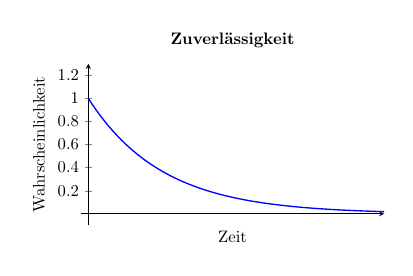
\begin{tikzpicture}
        [
            scale = 0.6,
            >=latex
        ]
        \begin{axis}
            [
                title=\textbf{Zuverlässigkeit},
                width=8cm,
                height=5cm,
                xmin=-0.2, xmax=8, ymin=-0.1, ymax=1.3, axis lines=middle,
                x label style={at={(axis description cs:0.5,0)},anchor=north},
                y label style={at={(axis description cs:-0.1,0.5)},rotate=90,anchor=south},
                xlabel=Zeit,
                ylabel=Wahrscheinlichkeit,
                xtick=\empty,
                ytick={0, 0.2, 0.4, 0.6, 0.8, 1, 1.2}
                %grid
            ]
        
            % plot
            \addplot[color=blue, thick, domain=-0:10]{exp(-0.5*x)};
        \end{axis}
        
    \end{tikzpicture}
\end{center}
\end{minipage}
\hfill
\begin{minipage}[c]{0.5\columnwidth}
    \raggedright

    \begin{itemize}
        \item Je länger das System läuft, desto weniger zuverlässig ist es
        \item Die Wahrscheinlichkeit für einen Ausfall steigt stetig
    \end{itemize}
    
    \vspace{0.2cm}

    \textbf{Achtung:} Hier ist nur die Alterung der Hardware berücksichtigt
\end{minipage}


\subsection{Verfügbarkeit}

Die Verfügbarkeit A (Availability) ist der Anteil der Betriebsdauer innerhalb dessen das System seine Funktion erfüllt.
$$ \text{Verfügbarkeit} = \frac{\text{Gesamtzeit} - \text{Ausfallzeit}}{\text{Gesamtzeit}} $$


% \subsection{Abstraktionsschichten}

% \begin{itemize}
%     \item Bei $\micro$C-Programmierung (Firmware) müssen oft Bitmuster in Register geschrieben werden
%     \item Solche Register-Zugriffe dürfen \textbf{nicht} 'willkürlich' überall im Code erfolgen \\
%         \textrightarrow\ schlecht lesbar, schlecht portiertbar, fehleranfällig
%     \item \textbf{Damit Code lesbarer und besser auf andere Platform portierbar wird, beinhaltet jeder professionelle Code einen
%         Hardware Abstraction Layer (HAL)}
%     \item HAL führt \textbf{nicht} zum Verlust bei Laufzeit, wenn korrekt implementiert
% \end{itemize}


% \subsubsection{Hardware-abstraction-layer (HAL)}

% \begin{itemize}
%     \item Trennt HW-Implementierung von SW-Logik
%     \item Gleiche SW kann auf verschiedene HW verwendet werden \textrightarrow\ Portabilität
%     \item HW-Komponenten können einfach ausgetauscht werden \textrightarrow\ Flexibilität
% \end{itemize}

